\chapter{Machine learning}


Qui verranno inserite tutte le brevi digressioni e cenni sul machine learning...



\section{NN: Neural Networks}

\begin{abstract}
Le NN sono modelli per il machine learning costruiti usando principi dell'organizzazione neuronale: un gruppo di nodi interconnesso(neuroni) che si trasmettono segnali.
Una rete neurale impara processando esempi contenenti un input ed un risultato noto/atteso per quell'input, costruendo associazioni probabilistiche e pesate, conservate nella struttura dati stessa  della rete.
Un neurone (artificiale) è una funziona matematica che riceve un input ne esegue una "somma" (con bias) e restituisce un output (es: sigmoid, step func, ...).
\end{abstract}
\begin{figure}
    \centering
    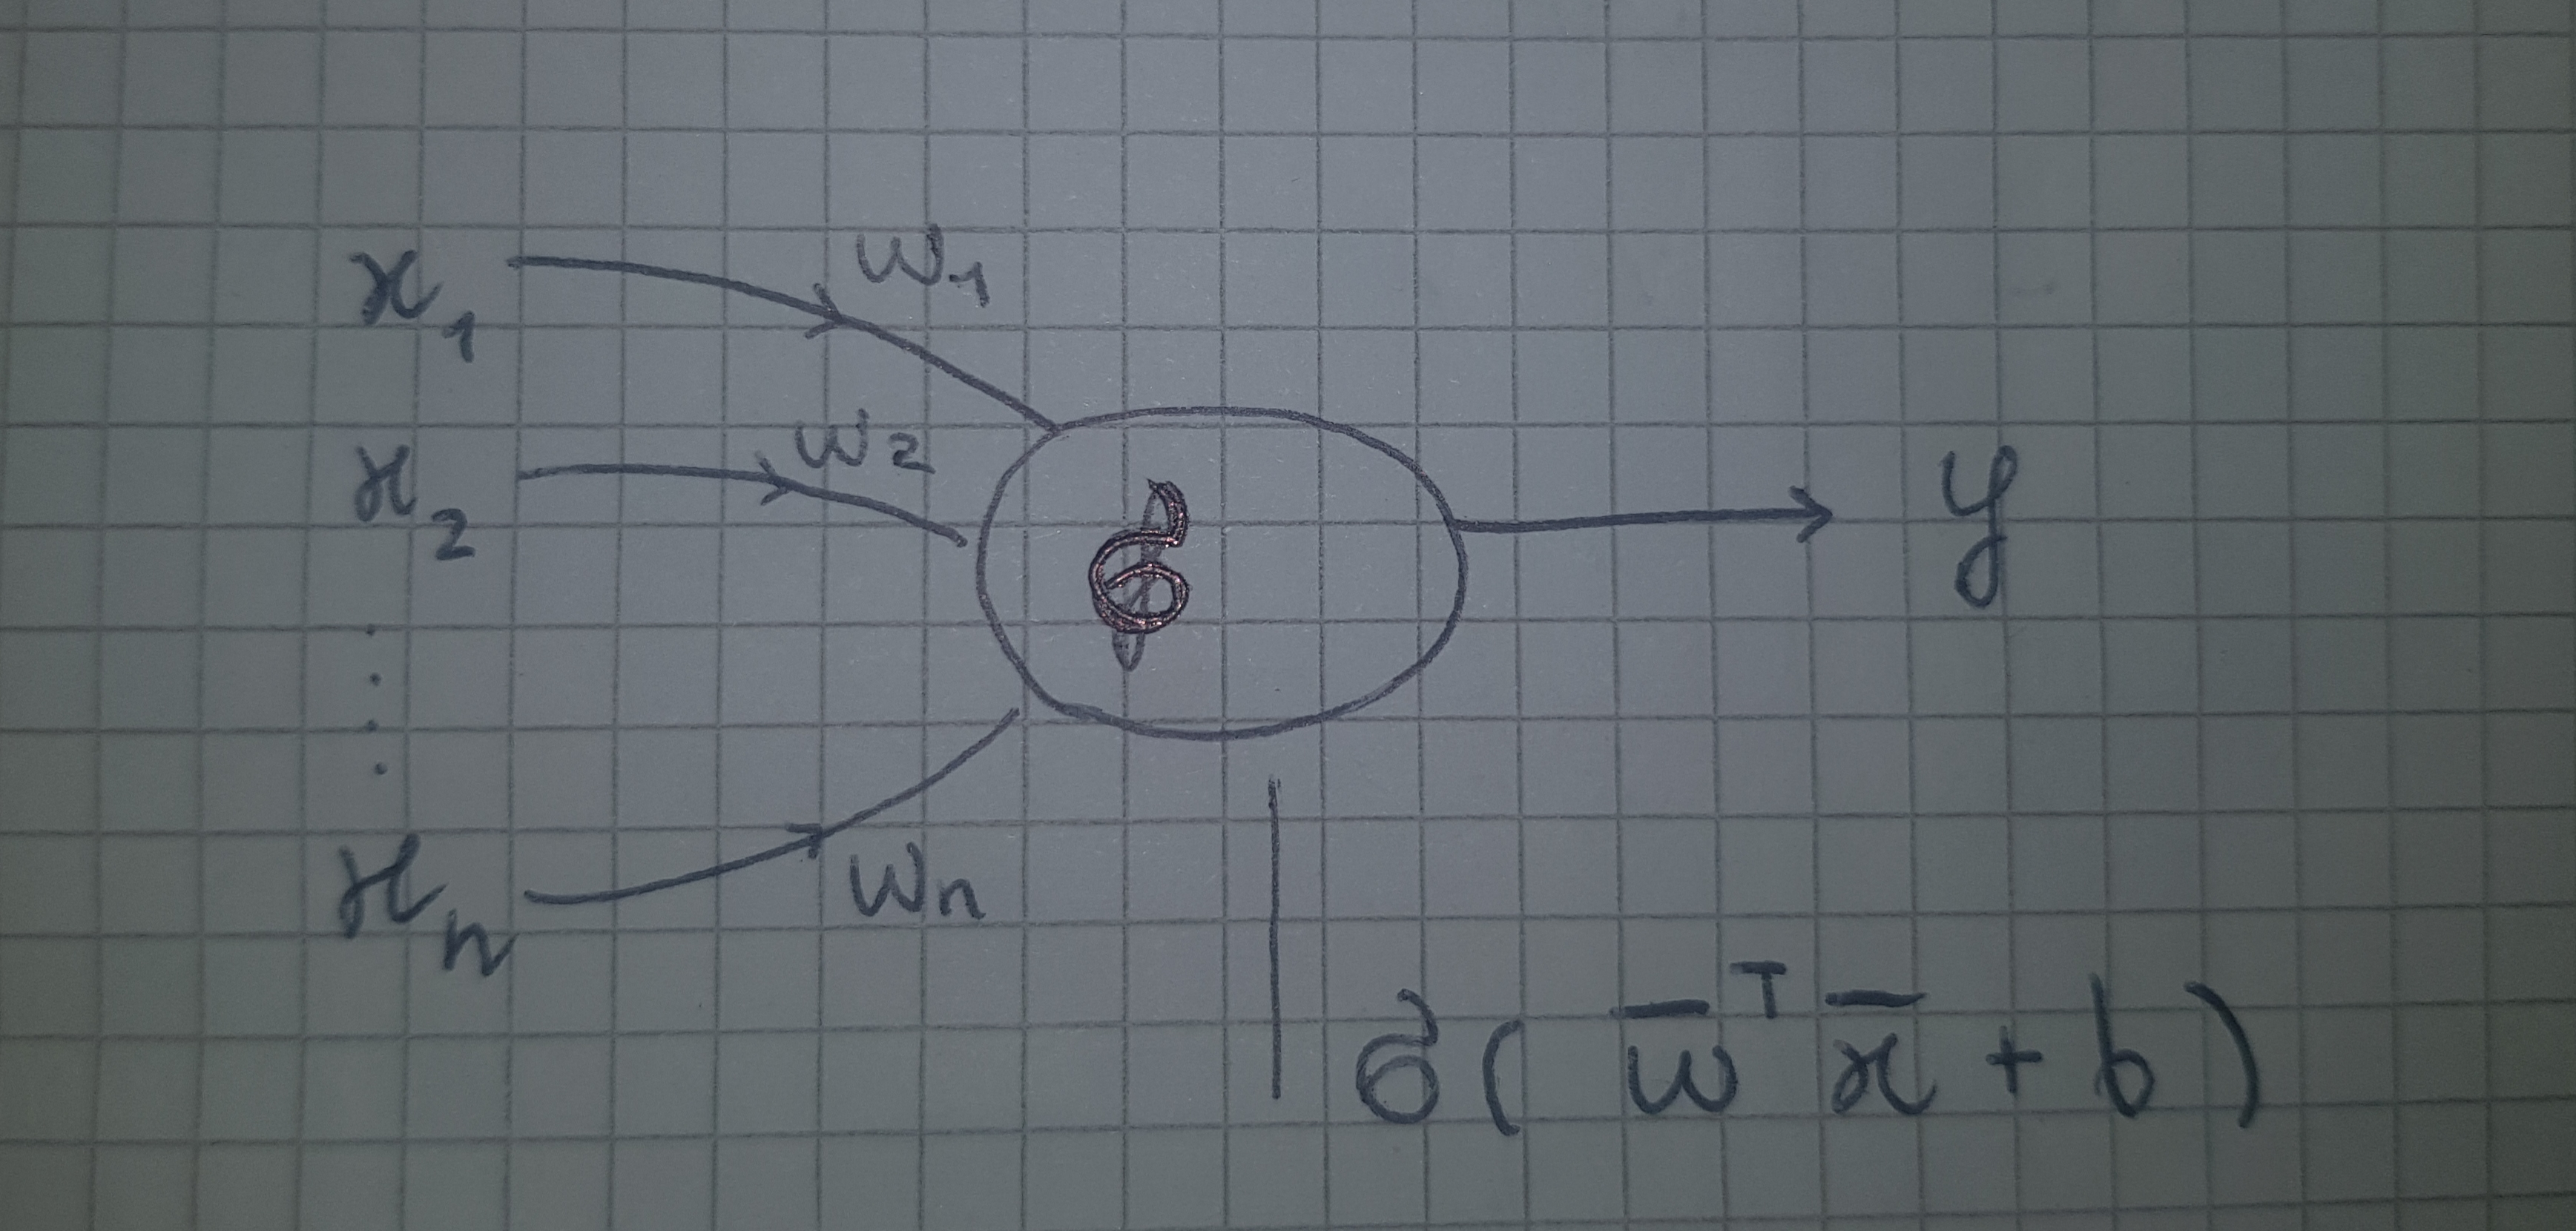
\includegraphics[width=0.5\linewidth]{20231130_172209.jpg}
    \caption{Enter Caption}
    \label{fig:enter-label}
\end{figure}